\documentclass[final]{beamer}
\usepackage[orientation=landscape,size=a0,scale=1.0]{beamerposter}
\usepackage[T1]{fontenc}
\usepackage{helvet}
\usepackage{mathptmx}
\usepackage{courier}
\usepackage{amsmath,amssymb,graphicx,array,colortbl,booktabs,tikz}
\usetikzlibrary{arrows.meta,positioning,calc}
\renewcommand{\familydefault}{\sfdefault}
\graphicspath{{../report/figures/}{assets/}{./}}
\definecolor{ink}{HTML}{251F21}
\definecolor{muted}{HTML}{585254}
\definecolor{teal}{HTML}{1F78B4}
\definecolor{pale}{HTML}{EDF4F9}
\definecolor{sand}{HTML}{F4EFEC}
\definecolor{rulecol}{HTML}{DCDDD9}
\setbeamercolor{normal text}{fg=ink,bg=white}
\setbeamertemplate{navigation symbols}{}
\setbeamertemplate{headline}{}
\setbeamertemplate{footline}{}
\setbeamersize{text margin left=0pt,text margin right=0pt}
\setlength{\parindent}{0pt}

\setlength{\parskip}{5pt}
\newcommand{\bodyfont}{\fontsize{21}{26}\selectfont}
\newcommand{\smallfont}{\fontsize{18.5}{23}\selectfont}
\newcommand{\capfont}{\fontsize{16}{20}\selectfont\color{muted}}
\newcommand{\heading}[2]{{\fontsize{26}{30}\selectfont\bfseries\color{teal} #1\quad #2}\par\vspace{2mm}{\color{rulecol}\hrule height 1.1pt}\vspace{3mm}}
\newcommand{\para}[2]{\textbf{#1} #2\par}
\newcommand{\place}[4]{\node[anchor=north west,inner sep=0pt,text width=#3cm] at ([xshift=#1cm,yshift=-#2cm]current page.north west) {\begin{minipage}[t]{#3cm}\bodyfont\raggedright #4\end{minipage}};}
\newcommand{\metric}[4]{\place{#1}{8.5}{#2}{{\fontsize{39}{43}\selectfont\bfseries\color{teal}#3}\par{\fontsize{21}{26}\selectfont #4}}}
\hypersetup{pdftitle={Lithium-Ion Battery SOH Estimation via Wide-and-Deep Sparse GPR with Uncertainty-Weighted Symbolic Residuals},pdfauthor={Divya Swaroop Jaiswal},pdfsubject={Research poster: battery health, sparse Gaussian processes and symbolic residuals}}
\begin{document}
\begin{frame}[t]
\begin{tikzpicture}[remember picture,overlay]
\fill[ink] (current page.north west) rectangle ([yshift=-7.2cm]current page.north east);
\fill[teal] ([yshift=-7.2cm]current page.north west) rectangle ([yshift=-7.5cm]current page.north east);
\place{2.2}{0.75}{114.5}{{\fontsize{17}{20}\selectfont\bfseries\color{white!70} WD-GPR-SR\hfill MACHINE LEARNING / RESEARCH POSTER}\par\vspace{2mm}
{\fontsize{46}{51}\selectfont\bfseries\color{white} Lithium-Ion Battery SOH Estimation via Wide-and-Deep Sparse GPR\par with Uncertainty-Weighted Symbolic Residuals}\par\vspace{3mm}
{\fontsize{23}{28}\selectfont\color{white} \textbf{Divya Swaroop Jaiswal}\quad /\quad 2401CS38\quad /\quad B.Tech CSE, IIT Patna\hfill\texttt{divya\_2401cs38@iitp.ac.in}}}
\fill[pale] ([xshift=2.2cm,yshift=-7.95cm]current page.north west) rectangle ([xshift=-2.2cm,yshift=-12.9cm]current page.north east);
\metric{3.2}{24}{4.854 $\pm$ 0.495}{RMSE, SOH percentage points}
\metric{32.8}{25}{96.59 $\pm$ 2.08\%}{Coverage of nominal 95\% intervals}
\metric{63.0}{22}{47 cells / 6,124 cycles}{NASA, CALCE \& Mobile2Mobile; leave-one-cell-out}
\place{92.5}{8.5}{23}{{\fontsize{24}{29}\selectfont\bfseries Three-seed evidence}\par\smallfont Seeds 42, 43, 44; mean $\pm$ sample SD. Best seed is reported separately, not as the mean.}

% Column separators
\draw[rulecol,line width=1pt] ([xshift=40.1cm,yshift=-14cm]current page.north west)--([xshift=40.1cm,yshift=-79.7cm]current page.north west);
\draw[rulecol,line width=1pt] ([xshift=79.1cm,yshift=-14cm]current page.north west)--([xshift=79.1cm,yshift=-79.7cm]current page.north west);
% LEFT COLUMN
\place{2.2}{14.0}{36.3}{\heading{01}{Abstract and research question}
WD-GPR-SR targets \textbf{competitive accuracy with more inspectable predictions}: a Bayesian GP provides uncertainty, a symbolic term exposes the residual correction, and XAI audits feature contributions. Under 47-cell LOCO, its best-seed RMSE is 4.406 points versus 4.330 for SVR, with 98.32\% versus 57.45\% interval coverage under the reported interval constructions. Across three seeds, RMSE averages 4.854 points. The model is not best on every metric; its value is the combination of useful accuracy, uncertainty and auditable components. Physical edge benchmarking remains future work.
}
\place{2.2}{23.8}{36.3}{\heading{02}{Data, target and leakage controls}
\[\mathrm{SOH}=100\,Q_{\mathrm{discharge}}/Q_{\mathrm{nominal}}\]
\para{Benchmark.}{NASA Ames 18650 cells and CALCE CS2/CX2 cells; reported SOH range 10.02--128.45\%, mean 76.46\%. Mobile2Mobile is context only, not part of the 6,124-cycle benchmark.}
\para{24 inputs.}{15 numeric summaries: cycle order, seven voltage statistics, three current statistics and four temperature statistics; four temperature-missingness flags and five one-hot metadata features.}
\para{Isolation.}{Capacity, Coulomb integrals and cycle duration are excluded. In each outer fold, hold out one entire cell; fit imputation, scaling and models only on the other 46. Five inner cell folds produce out-of-fold residuals and select the correction.}
}
\place{2.2}{36.5}{36.3}{\heading{03}{Architecture: train offline, infer at the edge}
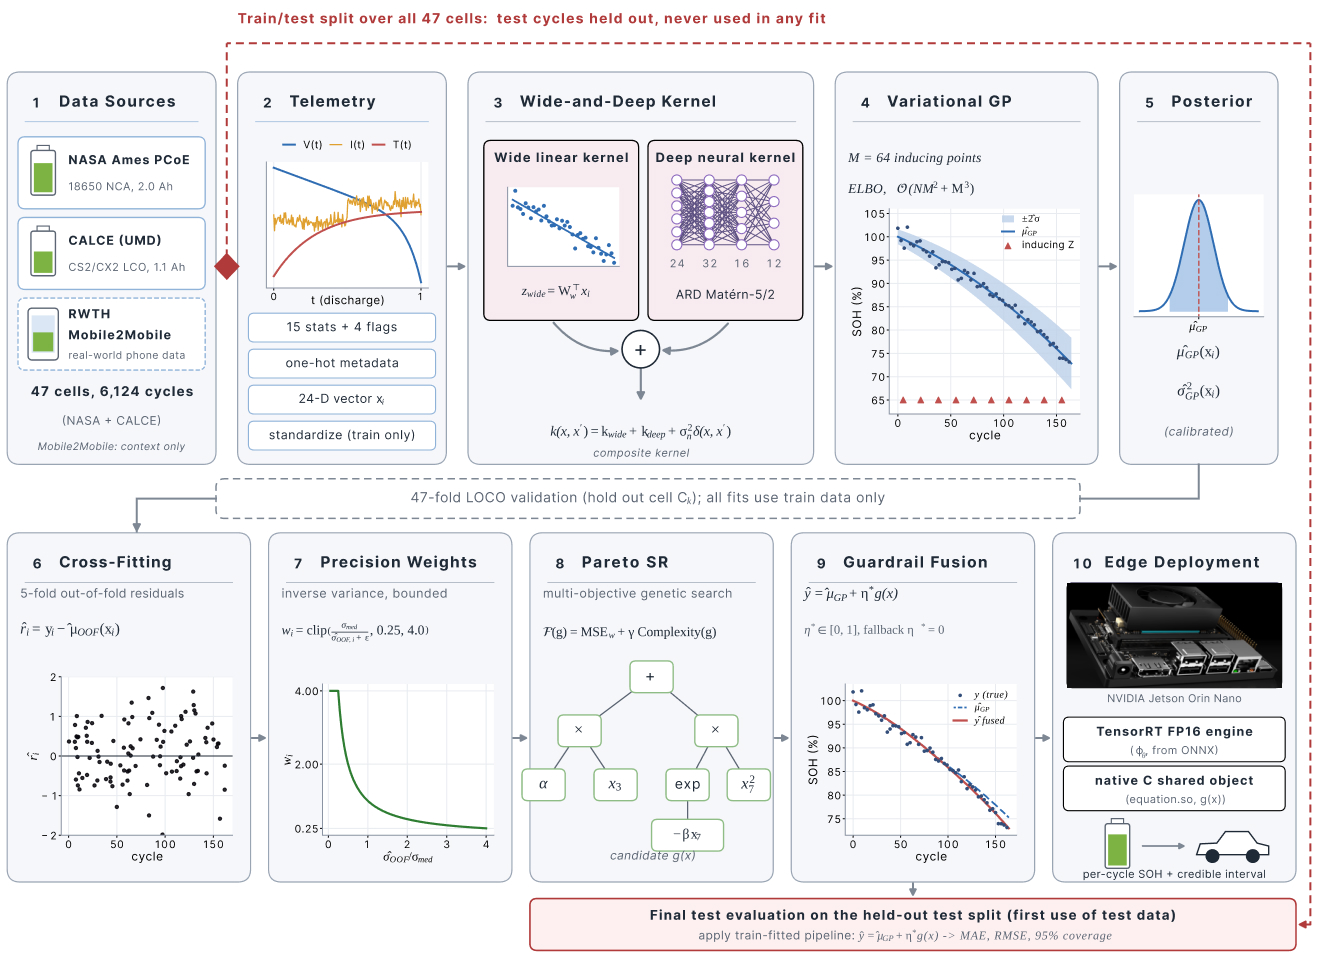
\includegraphics[width=\linewidth]{architecture.jpg}\par
{\capfont Original architecture figure from the report. Curves and example trees inside this diagram illustrate the workflow; numerical evaluation is reported separately. The equation uses inverse-SD weights despite the figure's inverse-variance label.}
}
\place{2.2}{66.8}{36.3}{\heading{04}{Model and optimization}
\smallfont
\[k(x,x')=k_{\mathrm{linear}}(x,x')+k_{\mathrm{deep}}(\phi_\theta(x),\phi_\theta(x'))\]
\[\mathcal L=\sum_i\mathbb E_{q(f_i)}\log p(y_i\mid f_i)-\mathrm{KL}(q(u)\Vert p(u))\]
\para{Scalability.}{Sparse cost $\mathcal O(NM^2+M^3)$ versus exact-GP $\mathcal O(N^3)$. Gaussian observation noise is modeled separately.}
\para{Settings reported.}{Adam 0.01; batch 256; 120 epochs maximum; patience 15; dropout 0.05. SR: population 160, 10 generations.}
\[w_i=\mathrm{clip}\!\left(\frac{\sigma_{\mathrm{med}}}{\sigma_{\mathrm{OOF},i}+10^{-6}},\,0.25,\,4\right)\]
\para{SR fitness.}{Minimize weighted residual MSE plus $0.002$ times expression node count. Weights use inverse standard deviation, not inverse variance.}
\para{Fusion.}{Validation selects $\eta\in[0,1]$ in steps of 0.05; reject SR if RMSE gain is below $10^{-4}$.}
}
% CENTER COLUMN
\place{41.7}{14.0}{35.8}{\heading{05}{Reported LOCO benchmark}
{\smallfont All entries transcribed from report Table 4. RMSE/MAE and interval width are in SOH percentage points. Lower error/NLL is better; coverage must be read alongside width.}\par\vspace{3mm}
{\fontsize{19}{24}\selectfont\setlength{\tabcolsep}{5pt}\renewcommand{\arraystretch}{1.14}
\begin{tabular*}{\linewidth}{@{\extracolsep{\fill}}lrrrrr@{}}
\toprule
\textbf{Model} & \textbf{MAE} & \textbf{RMSE} & \textbf{NLL} & \textbf{PICP\%} & \textbf{Width}\\\midrule
SVR & 2.932 & \textbf{4.330} & 7.878 & 57.45 & 4.64\\
\rowcolor{pale} WD-GPR-SR, seed 42 & 3.082 & 4.406 & 3.006 & 98.32 & 25.23\\
Deep NN & 3.063 & 4.517 & 6.644 & 55.94 & 5.24\\
Wide + deep NN & 3.413 & 4.696 & 8.015 & 48.99 & 4.94\\
GPR Mat\'ern & 3.005 & 4.757 & 3.388 & 76.68 & 14.31\\
Wide NN & 3.367 & 4.863 & 7.237 & 57.04 & 5.57\\
BiLSTM & 3.361 & 4.877 & 11.871 & 47.26 & 4.19\\
Sparse GPR & 3.469 & 4.988 & 3.102 & 82.54 & 11.76\\
Deep-kernel GPR & 3.571 & 5.265 & 3.244 & 99.40 & 33.41\\
XGBoost & 4.027 & 6.232 & 10.905 & 52.11 & 5.63\\
GPR RBF & 3.661 & 6.495 & 3.346 & 79.72 & 15.55\\
GPR ARD & 4.060 & 6.596 & 3.342 & 74.74 & 14.29\\
Random Forest & 4.007 & 6.772 & \textbf{2.990} & 93.22 & 21.25\\
Standalone SR & 8.886 & 12.345 & 3.934 & 94.01 & 44.64\\\midrule
\rowcolor{pale} WD-GPR-SR, 3-seed mean & 3.273 & 4.854 & 3.074 & 96.59 & 25.93\\\bottomrule
\end{tabular*}}
\vspace{3mm}\smallfont
\textbf{Reading the trade-off.} SVR has the best point RMSE; the report's residual-based SVR intervals under-cover. WD-GPR-SR trades wider intervals for higher coverage. RF has the lowest tabulated NLL. Baseline multi-seed uncertainty is not supplied, so a best-seed ranking is not a significance test.
}
\place{41.7}{38.6}{35.8}{\heading{06}{Prediction and uncertainty diagnostics}
\begin{minipage}[t]{0.485\linewidth}\vspace{0pt}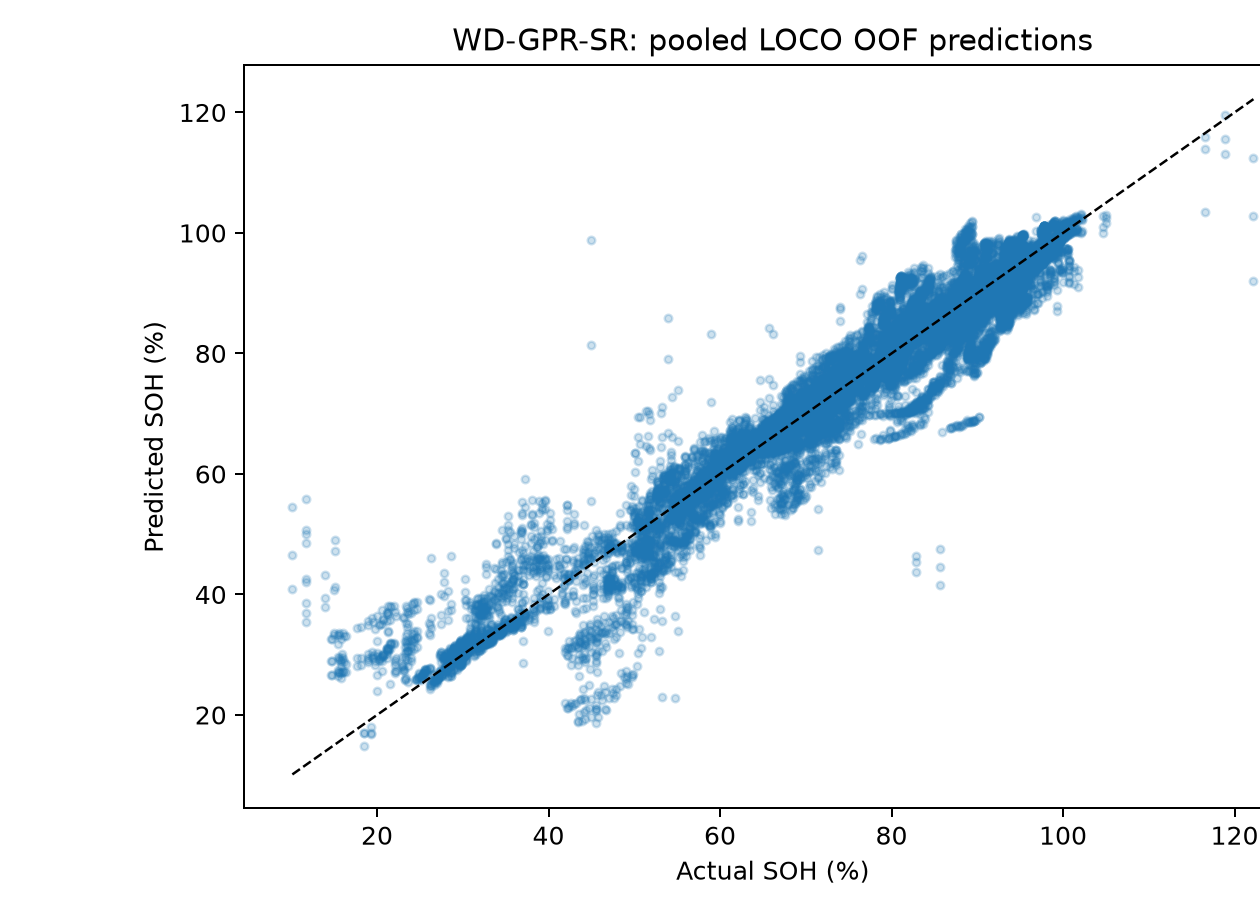
\includegraphics[width=\linewidth]{loco_pred_vs_true.png}\end{minipage}\hfill\begin{minipage}[t]{0.485\linewidth}\vspace{0pt}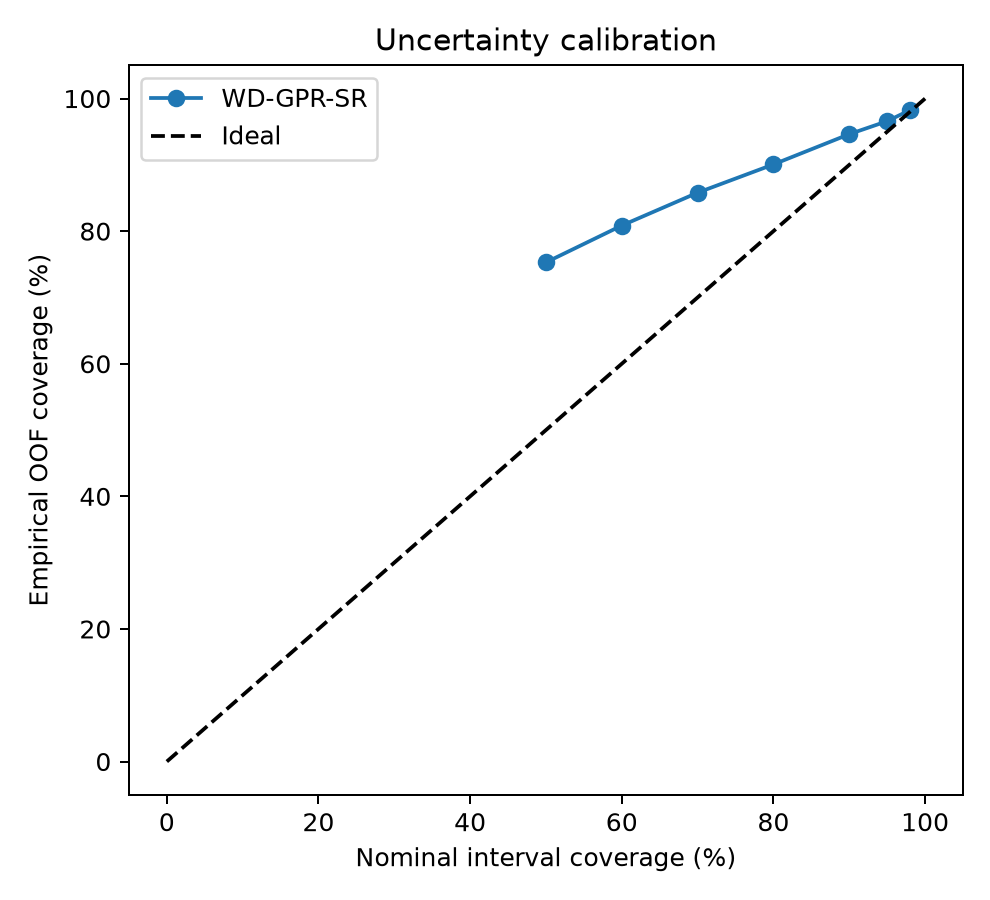
\includegraphics[width=\linewidth]{uncertainty_calibration.png}\end{minipage}\par\vspace{2mm}
\begin{minipage}[t]{0.485\linewidth}\vspace{0pt}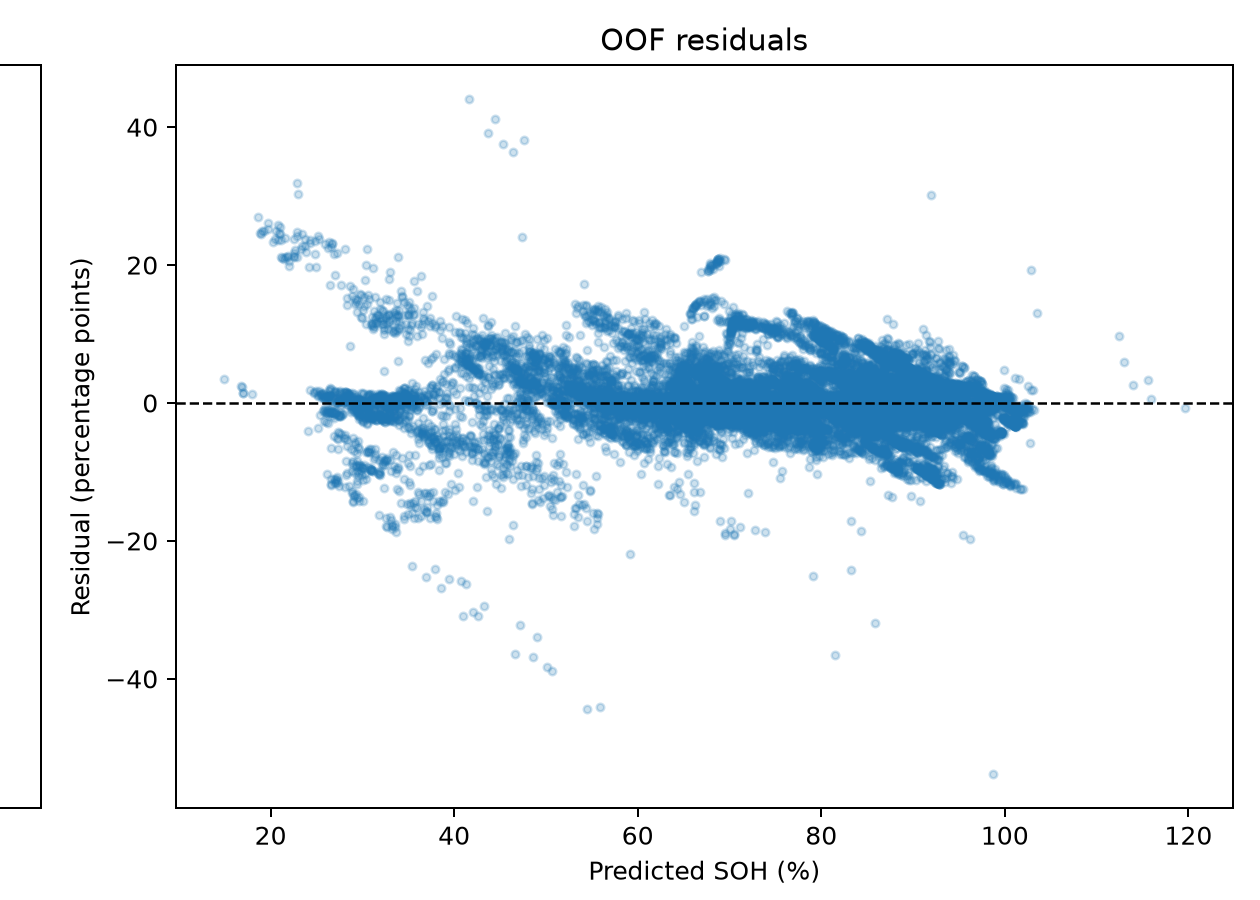
\includegraphics[width=\linewidth]{loco_residuals.png}\end{minipage}\hfill\begin{minipage}[t]{0.485\linewidth}\vspace{0pt}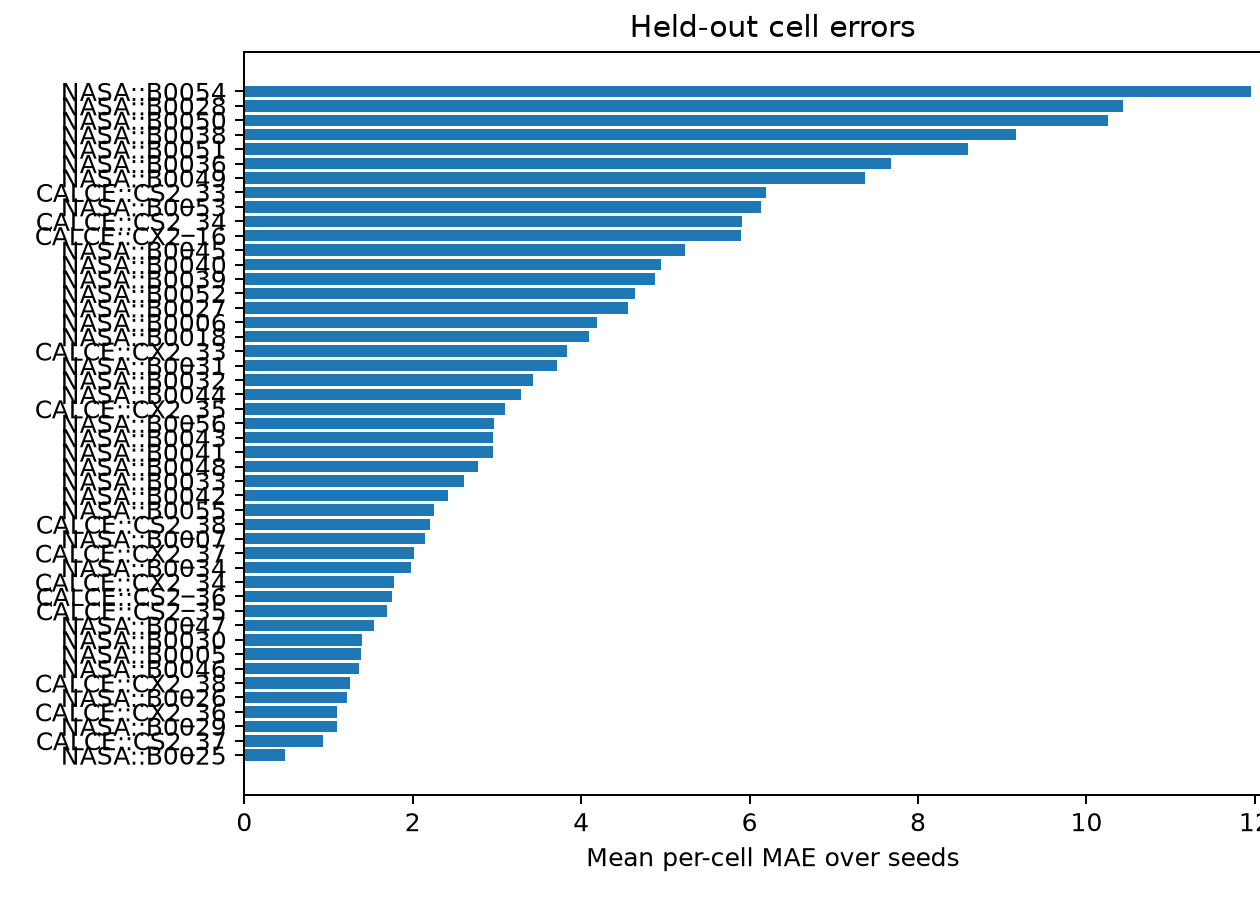
\includegraphics[width=\linewidth]{loco_cell_mae.png}\end{minipage}\par
{\capfont Unchanged report plots: pooled prediction, calibration, residuals and held-out-cell MAE. Coverage is conservative at lower nominal levels. Outliers and uneven cell errors limit what pooled metrics prove; test cell-wise coverage and chemistry shift next.}
}
\place{41.7}{71.2}{35.8}{\heading{07}{Seed stability, not best-seed selection}
{\fontsize{19}{23}\selectfont\setlength{\tabcolsep}{9pt}\renewcommand{\arraystretch}{1.15}
\begin{tabular*}{\linewidth}{@{\extracolsep{\fill}}lrrrr@{}}\toprule
 & \textbf{42} & \textbf{43} & \textbf{44} & \textbf{Mean $\pm$ SD}\\\midrule
RMSE & 4.406 & 5.385 & 4.771 & $4.854\pm0.495$\\
MAE & 3.082 & 3.490 & 3.248 & $3.273\pm0.205$\\
$R^2$ & 0.9383 & 0.9078 & 0.9276 & $0.9246\pm0.0155$\\
PICP (\%) & 98.32 & 94.28 & 97.16 & $96.59\pm2.08$\\
\bottomrule\end{tabular*}}
\vspace{3mm}\smallfont
\para{Other means.}{MSE $23.725\pm4.864$; MAPE $5.370\pm0.441\%$; NLL $3.074\pm0.073$; width $25.93\pm0.64$ points. Seed 43 under-covers at 95\%.}

}
% RIGHT COLUMN
\place{80.7}{14.0}{36.0}{\heading{08}{Ablation: what actually helps?}
\begin{center}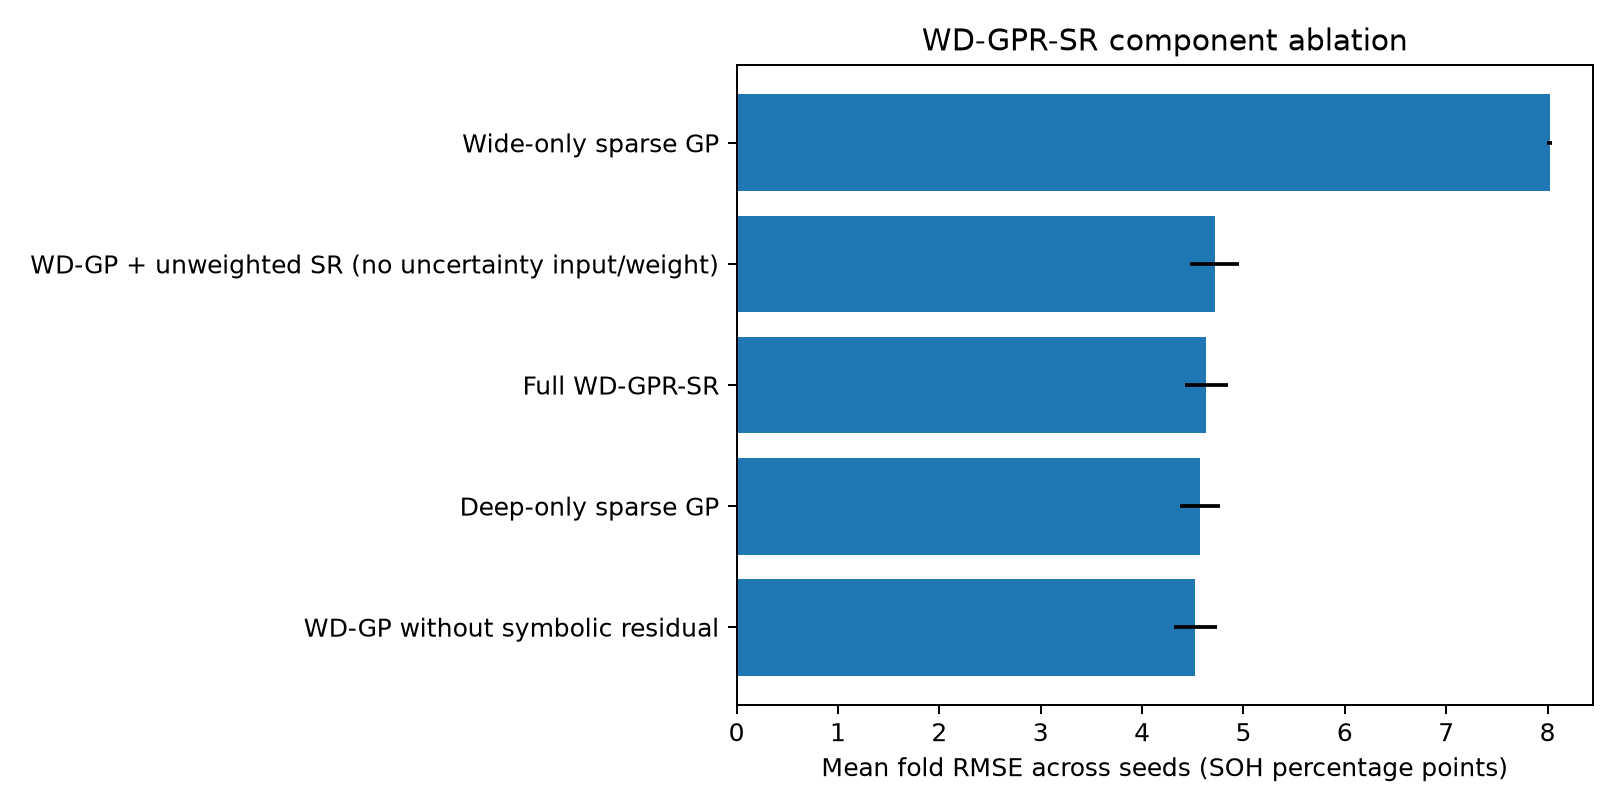
\includegraphics[width=0.57\linewidth]{ablation_rmse.png}\end{center}\par
{\capfont Report ablation plot; separate from the main seed table.}\par\vspace{2mm}\smallfont
\textbf{RMSE:} wide-only 8.019; deep-only 4.575; WD-GP without SR \textbf{4.525}; unweighted SR 4.716; weighted SR 4.633.
\par Weighted SR improves on unweighted SR, but \textbf{neither beats no SR}. The deep branch is essential; the wide branch adds only a small gain.
}
\place{80.7}{31.0}{36.0}{\heading{09}{Multi-criteria profile: report spider chart}
\begin{center}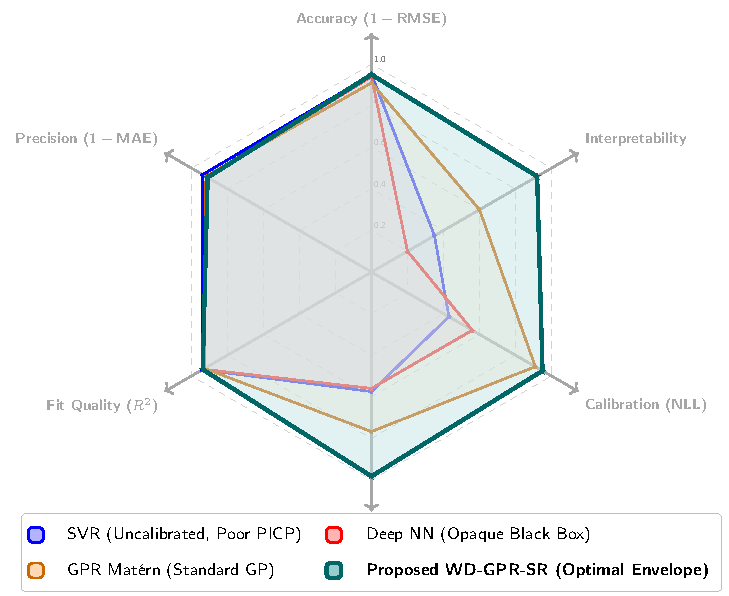
\includegraphics[width=22.5cm]{spider_chart.pdf}\end{center}
{\capfont Original vector chart cropped from report Figure 2. This is an illustrative normalized profile: the report does not give a reproducible scaling rule or a measured interpretability score. Use the benchmark table for numerical comparisons.}
}
\place{80.7}{54.3}{36.0}{\heading{10}{Explainability and the discovered equation}
\begin{minipage}[t]{0.47\linewidth}\vspace{0pt}
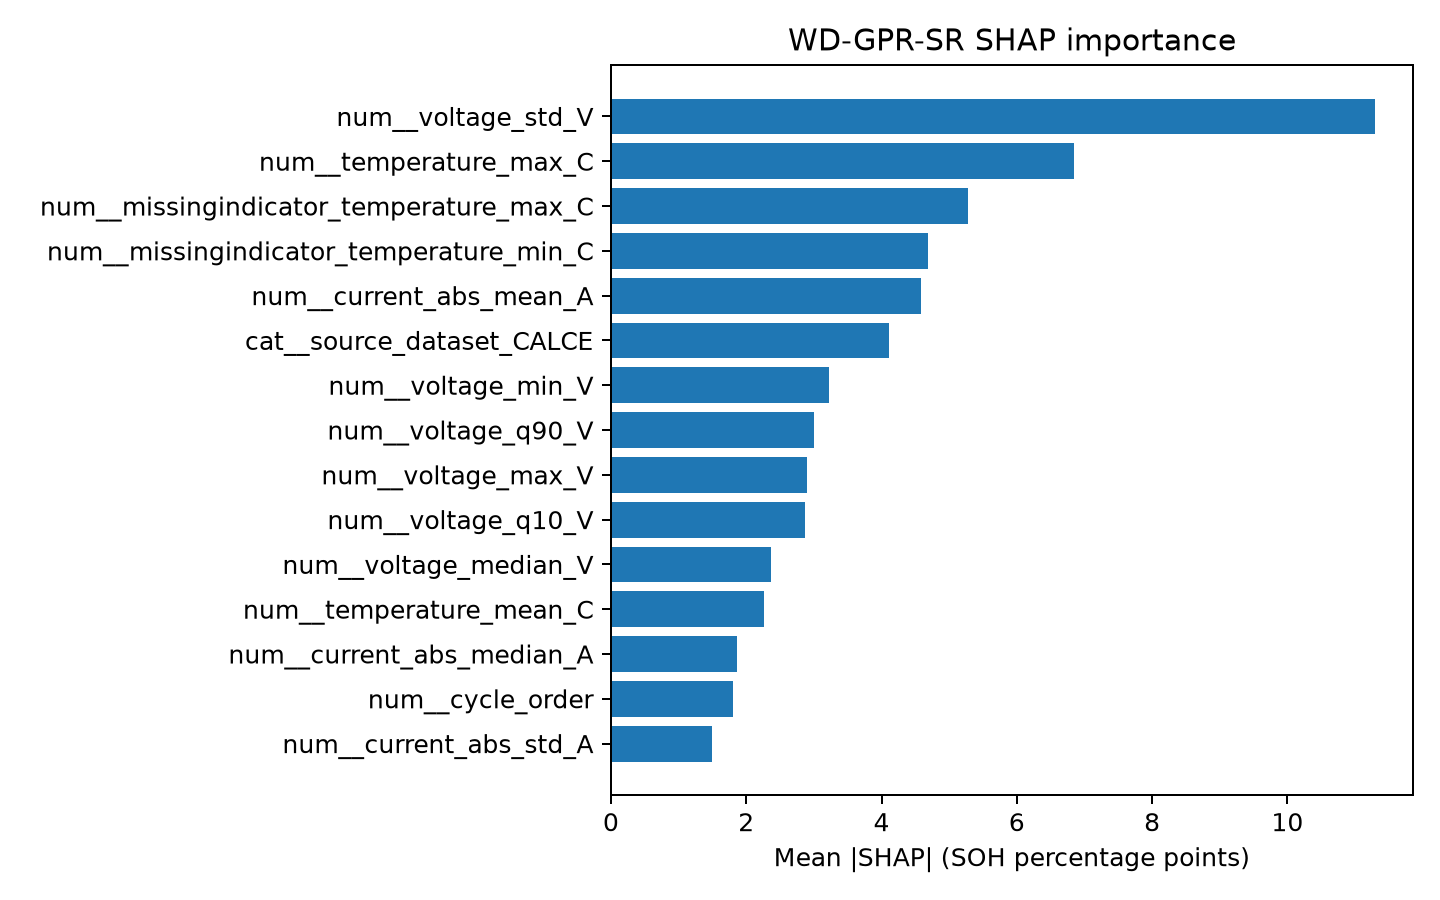
\includegraphics[width=\linewidth]{shap_importance.png}
\end{minipage}\hfill\begin{minipage}[t]{0.50\linewidth}\vspace{0pt}\smallfont
\textbf{SHAP leaders}\par Voltage SD: 11.292\par Peak temperature: 6.852\par Missing-temperature flags also rank highly, suggesting possible dataset/sensor shortcuts.\par\vspace{2mm}{\capfont Attributions are associations, not causal proof.}
\end{minipage}\par\vspace{2mm}\smallfont
\para{Other report audits.}{LIME gives a local surrogate; PDP and ICE inspect responses; ARD ranks latent dimensions. Standardized LIME thresholds must not be read as physical amperes or degrees.}
\[g(x)=-(-0.061094)\simeq0.0611,\qquad\partial g/\partial x_j=0\]
\textbf{Interpretation.} A constant offset in standardized target units (about 1.08 SOH points before shrinkage), not a physical aging law or proof that the GP learned all mechanisms.
}
\place{80.7}{72.4}{36.0}{\heading{11}{Edge plan and next experiments}
\smallfont
\textbf{Translation plan:} PyTorch $\to$ ONNX $\to$ TensorRT FP16; sparse-GP arrays and precomputed weights; symbolic term compiled to C.\par
\textbf{Pending measurements:} at least 1,000 warmed-up Jetson runs, p50/p95 latency, peak memory, power and energy/inference, with precision and power mode. No physical measurements are supplied.\par
\textbf{Next:} matched-seed baselines, per-cell calibration, chemistry/temperature shift and missingness audits. Competitive accuracy plus inspection tools, not an all-metric winner or safety-validated BMS.
}
% FOOTER
\draw[rulecol,line width=1.3pt] ([xshift=2.2cm,yshift=-80.5cm]current page.north west)--([xshift=-2.2cm,yshift=-80.5cm]current page.north east);
\place{2.2}{81.0}{114.5}{\fontsize{15}{19}\selectfont\color{muted}
\textbf{Sources and scope.} Project report, \texttt{report/main.tex}, Tables 4--8 and supplied figures; PBL brief and IMPACT Lab guidelines. Dataset sources: NASA Ames PCoE and CALCE (University of Maryland). Method references cited in report: Titsias, AISTATS (2009), sparse variational GP; Cranmer, arXiv:2305.01582 (2023), symbolic regression.\par
Poster summarizes supplied results; experiments were not rerun. Metrics are kept distinct across benchmark, seed and ablation experiments. All measured plots and the architecture are reused unchanged. The spider chart is an illustrative profile from report Figure 2.}
\end{tikzpicture}
\end{frame}
\end{document}
